\section{Demo interface}
\label{sec:demo-interface}

AutoTerm-SST serves listeners of specialized live speech who cannot prepare a
glossary for every session, such as conference attendees, students in
technical courses, and clinicians following medical lectures. The demo starts
like an ordinary streaming translator: the user selects a language pair and
starts a microphone or file stream, with no glossary upload or domain
selector.

\paragraph{Walkthrough.}
A session follows topic changes with no manual control. Partial translations
appear immediately; once context accumulates, the slice status row switches to
the highest-scoring slices, and retrieved pairs appear beside the output that
used them. After a topic change, outgoing and incoming slices briefly
coexist.

\begin{figure*}[t]
  \centering
  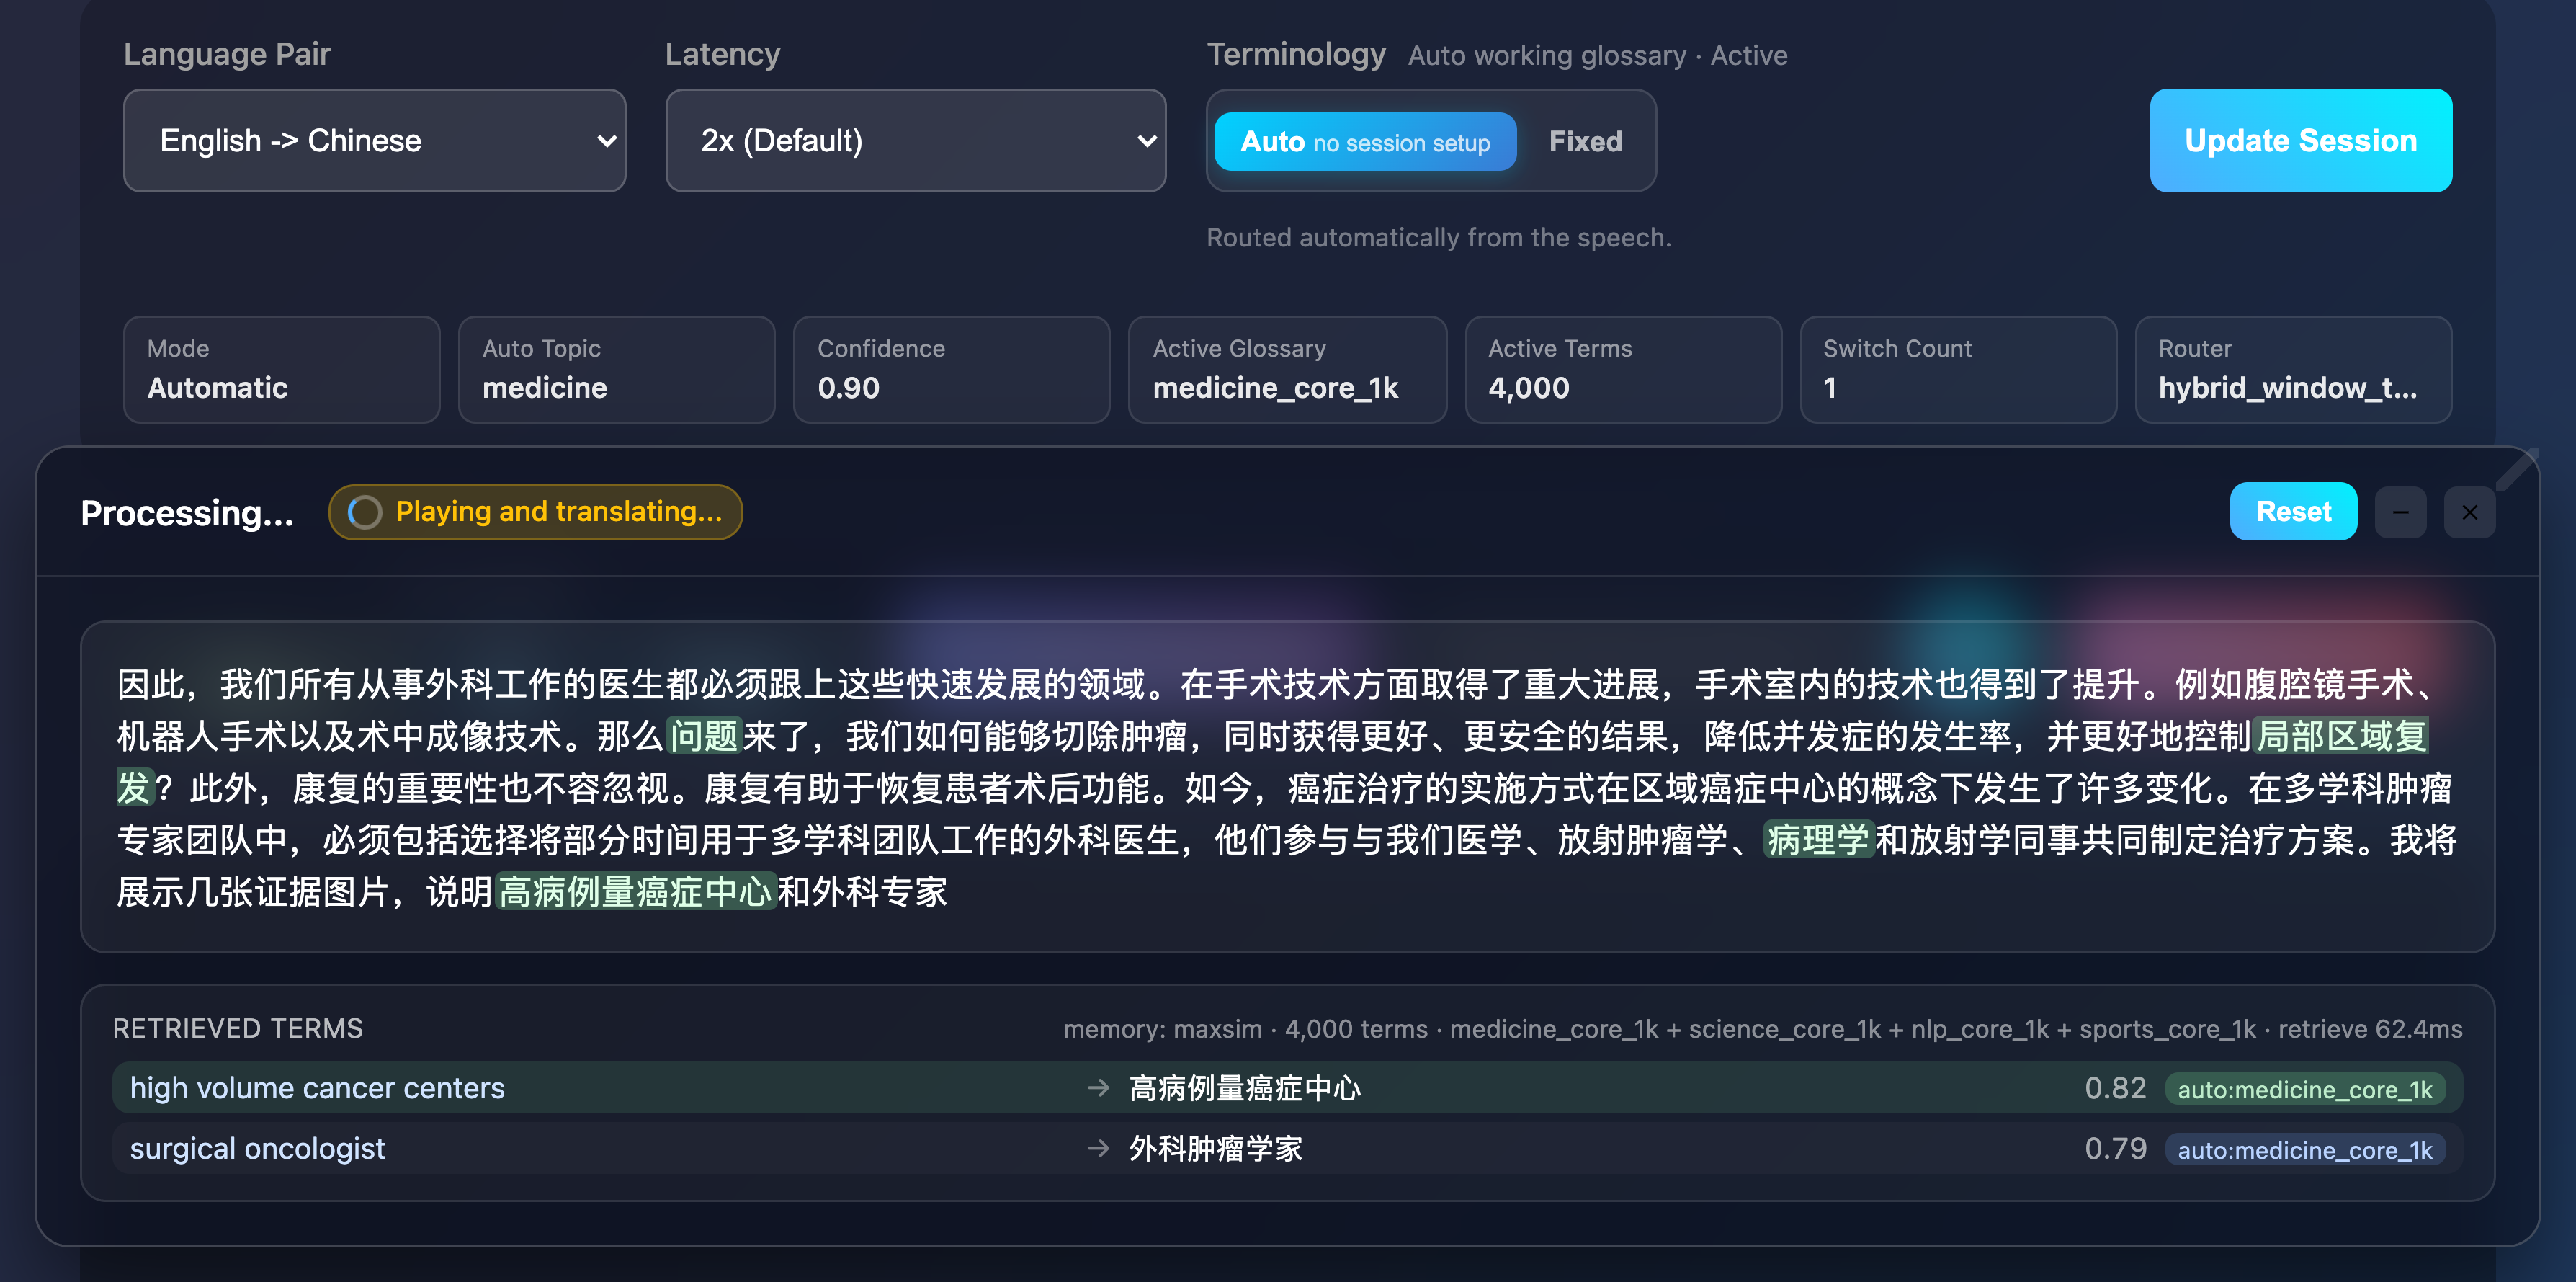
\includegraphics[width=0.72\textwidth]{ui_evidence_panel.png}
  \caption{The English-to-Chinese interface during an oncology lecture, replaying
  the recorded outputs of run 1 about 20 minutes into the stream. The status row
  shows the confirmed medicine slice and the 4,000 searchable terms, retrieved
  terms are highlighted in the translation, and the bottom panel lists the latest
  retrieved term pairs with their scores and source slices.}
  \label{fig:ui}
\end{figure*}

\paragraph{Visible terminology evidence.}
Inline term highlighting and a dedicated evidence panel make terminology
behavior transparent during streaming. As Figure~\ref{fig:ui} shows, the
interface highlights retrieved terms inside the translation, lists their
source--target mappings, and displays the active slices, active term count, and
retrieval latency in a status row. Viewers can directly determine whether a
mistranslation stems from missing retrieval evidence, an irrelevant slice, or
LLM decoding.

\paragraph{Extensibility.}
Organizations grow the catalog from single glossary files without restarting
the service. Registration validates the term pairs, builds an independent
MaxSim index, and writes one manifest entry. Prototypes can be written by hand
or generated from the glossary by an LLM, and Appendix~\ref{app:router} shows
that generated prototypes route as accurately. Running sessions keep their
snapshot while new sessions see new slices at once, and fixed-glossary presets
remain available for expert users.

\paragraph{Availability.}
The MIT-licensed implementation, a one-command launcher, and a screencast are
in the \href{https://github.com/luojiaxuan/autoterm-sst}{GitHub repository},
and the hosted entry page is \url{https://luojiaxuan.github.io/autoterm-sst/}.
Live mode serves Qwen3-Omni with vLLM continuous batching alongside the RASST
retriever.
